\chapter{Materiales y métodos}
\newcommand{\ros}{\texttt{ROS} }
\section{\ros}
\ros (Robot Operative System) \cite{ros} es un sistema operativo de código abierto basado en paso de mensajes diseñado para plataformas robóticas. Sus usos van desde el diseño de drivers, a resolver problemas complejos como la navegación autónoma.

La filosofía del sistema operativo es permitir a los desarrolladores abarcar de manera independiente los problemas que surgen al desarrollar una plataforma robótica, de modo que cada módulo pueda comunicarse con el resto, y que no haya que rediseñar un programa cuando se quiere cambiar de plataforma (y que una misma plataforma se beneficie de la implementación de distintos programas).

La versión usada para trabajar con el robot Baxter \cite{baxter} ha sido \texttt{Indigo}, ya que es la versión soportada por el robot.
\subsection{Arquitectura}
La arquitectura de \ros sigue un modelo distribuido, donde cada nodo realiza una tarea y los nodos pueden comunicarse entre sí. Esta comunicación lo hace mediante paso de mensajes.
\subsubsection{Nodos}
Los nodos son los programas que realizan las tareas, ejecutables que utilizan \ros para comunicarse con otros nodos. Para programarlos se usan las librerías \textit{roscpp} (para c++) o \textit{rospy} (para Python). En el presente trabajo se utiliza la implementación en Python (por motivos de compatibilidad con la interfaz de programación de aplicaciones (API) de Baxter, así como con las librerías \textit{tensorflow} \cite{tensorflow} y \textit{keras} \cite{keras} explicadas más adelante).

\subsubsection{Temas}
Los temas son los canales de comunicación que utilizan los nodos para comunicarse con otros nodos. Son los ``puertos'' que cada tema pone hace público para permitir la comunicación con otros nodos.

Los nodos publican y se suscriben a los temas.

\subsubsection{Mensajes}
La comunicación entre nodos se hace con el paso de mensajes. Estos son estructuras de datos que permiten a los nodos especificar y conocer la información que envían y reciben.

\subsubsection{Servicios}
Se trata de otra manera de comunicación, en la que un nodo hace una petición a otro y éste puede responder. Se diferencia de los mensajes en que el suscriptor puede responder al mensaje recibido, y su uso está enfocado a tareas aperiódicas.

\subsubsection{Parámetros}
Los parámetros son piezas de información contenidas en cada nodo que pueden ser vistas y modificadas por los nodos.

\subsubsection{Ejemplo}
Como ejemplo, se puede pensar en una cámara de vídeo que retransmite el vídeo en tiempo real. Esta cámara es un nodo (\texttt{/camera}) que publica mensajes del tipo imagen (que consiste en una matriz de nxm píxeles) al tema \texttt{/camera/image}.

Por otro lado, en un servidor estamos ejecutando un programa de detección de imágenes haciendo uso de \ros para la comunicación (nodo \texttt{/camera/server}). Este programa se suscribe al tema \texttt{/image} para recibir las imágenes que va a analizar.

Adicionalmente, la cámara tiene habilitado un servicio para reiniciar la cámara (\texttt{/camera/reset}) así como un conjunto de parámetros para filtrar las imágenes antes de publicarlas (\texttt{/color\_mode}), que permite cambiar la imagen a blanco y negro, sepia...

\subsection{\texttt{rosbag}}
\label{subsec:metodos/rosbag}
\texttt{rosbag} \cite{rosbag} es una herramienta para grabar el paso de mensajes realizados sobre los temas que se le ofrecen como parámetros. Tiene la capacidad de grabar información adicional a los mensajes, como la marca temporal (momento en el que el mensaje es registrado) y de secuencia (número de mensaje en una secuencia) que cada mensaje tiene asociada. Esto es útil para sincronizar mensajes generados por otro sistema y recibidos por tcp/ip con los mensajes generados en el propio ordenador.


\section{Baxter}
% Describir temas fundamentales
El robot biomórfico Baxter se trata de un robot de bajo coste (28.000 euros) y de baja fuerza, capaz de trabajar en entornos seguros, con otras personas a su alrededor. Esto se debe al uso de motores de bajo torque, así como del uso de actuadores elásticos en serie \cite{pratt1995series}.

Cuenta con un modelo de movimiento automático basado en aprendizaje de ejemplos dados por una persona, lo que permite a personal no cualificado enseñarle a realizar tareas.
\subsection{Hardware}
% Explicar hardware y software de Baxter (procesador, JCBs, ros, interfaz de comunicación (baxter.sh))
\subsubsection{Estructura física}
El robot cuenta con:

\begin{itemize}
\item [2 brazos] Con 7 articulaciones (grados de libertad) cada uno y sensores que miden la posición, velocidad y torque aplicado en cada una de las articulaciones.
\item [Pantalla] En la cabeza, con la capacidad de moverse hacia los lados.
\item [3 cámaras] Una al final de cada brazo y una en la pantalla, con una resolución máxima de 1280 x 800 píxeles y una tasa de refresco de 30 cuadros por segundo. 
\item [Pinzas] Que se colocan al final de cada articulación. También se puede colocar una bomba de vacío. No interfieren con las cámaras.
\item [Sonar] Ubicado en la cabeza.
\item [Botones] Para interactuar con el robot, ubicados en los brazos, así como en el torso, a cada lado del robot.
\end{itemize}

Las articulaciones son:

\begin{itemize}
\item[s0] Rotación del hombro.
\item[s1] Traslación del brazo.
\item[e0] Rotación del brazo.
\item[e1] Traslación del antebrazo.
\item[w0] Rotación del antebrazo.
\item[w1] Traslación de la mano.
\item[w2] Rotación de la muñeca, a fin de satisfacer dicho movimiento cuando la pinza se encuentra insertada.
\end{itemize}

Dichas articulaciones se pueden observar en la figura \ref{fig:desarrollo/joints}.

\begin{figure}[]
	\centering
	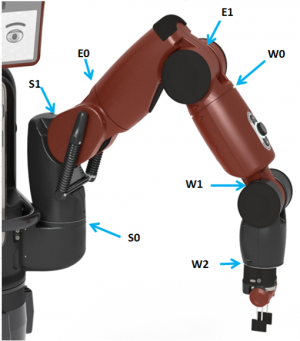
\includegraphics[width=2.5in]{imagenes/metodos/baxter_joint_names.png}
	\caption{Articulaciones del robot Baxter}
	\label{fig:desarrollo/joints}
\end{figure}

\subsubsection{Procesamiento}
En el interior del Baxter contamos con un procesador Intel Core i7-3770 a 3.4 GHz con tarjeta gráfica integrada, 4 GB de memoria RAM, y 128 GB de disco duro SSD.

\subsubsection{Actuadores elásticos en serie}
Los motores utilizados para las articulaciones utilizan actuadores elásticos en serie, en contraposición a los actuadores rígidos, usados en tareas de gran precisión.

Los actuadores rígidos basan su correcto funcionamiento en la cantidad de torque que pueden aplicar: a mayor torque, mayor precisión. Suelen ser controlados sin realimentación, y basan su control en un mapeo de voltajes y posiciones. Al tener tanto torque los motores, cualquier fuerza externa se vuelve despreciable, por lo que se puede confiar su control a uno basado en el conocimiento del motor.

Es este gran torque el que hace que los robots diseñados con estos motores no sean seguros para las personas. Los robots industriales en cadenas de montaje usan este tipo de actuadores.

Por otro lado, los actuadores elásticos basan su funcionamiento en la cantidad de torque que aplican, lo que significa que un controlador basado en realimentación es necesario, ya que el motor no conoce la posición en la que está, sino el torque que está aplicando. Esto lo consigue haciendo uso de elementos elásticos, los cuales aplican una fuerza sobre el objeto a mover. La posición de dicho objeto se mide y se transmite al controlador, que aplicará la fuerza correspondiente.

Los robots basados en estos actuadores son más seguros, ya que la cantidad de torque se puede controlar, ya sea por software o por la propia construcción hardware. Baxter utiliza este tipo de actuadores.

\subsection{Disposición}
Para trabajar con el robot se dispone de un laboratorio de dimensiones reducidas, teniendo en cuenta el rango de movimiento del robot y la compartición del espacio con más gente.

Además del robot, es necesario un equipo de trabajo, que consistirá en un ordenador de sobremesa con un procesador Intel Core i7-5930k a 3.5 GHz, 32 GB de memoria RAM y 200 GB de disco SSD y 1 TB de disco HDD.

Este equipo se usará para comunicarse con el robot, ejecutando el programa en el ordenador y transmitiendo mensajes entre el robot y éste haciendo uso de \ros.

\subsection{Modos de control}
Cada brazo se puede controlar de manera independiente, pudiendo usar cada uno de ellos con un modo de control distinto. Los modos de control son los que se muestran a continuación:

\begin{enumerate}
\item Control por posición
\item Control por velocidad
\item Control por torque
\item Control por posición sin procesar (raw mode)
\end{enumerate}

Haciendo uso de la arquitectura de paso de mensajes que nos ofrece \ros, somos capaces de enviar en un tema (topic) tanto el modo de control que queremos usar como las características objetivos que queremos en el movimiento. El robot Baxter estará escuchando cada uno de los mensajes que le enviemos a los temas \texttt{/robot/limb/left/joint\_command} para el brazo izquierdo y \texttt{/robot/limb/right/joint\_command} para el brazo derecho. El tipo de mensaje que se envía es \texttt{JointCommand}, que tiene como argumentos:

\begin{itemize}
\item mode (POSITION\_MODE=1, VELOCITY\_MODE=2,\\TORQUE\_MODE=3, RAW\_POSITION\_MODE=4)
\item command (lista de flotantes)
\item names (lista de nombre de articulaciones)
\end{itemize}

El modo de control para cada brazo es único, mientras que la posición/velocidad/torque deseado es único para cada articulación en cada brazo.

Aparte de enviar este tipo de mensajes, podemos definir la velocidad relativa máxima que alcanzará cada articulación en el modo de control por posición publicando al tema \texttt{/robot/limb/<right/left>/set\_speed\_ratio} un valor entre 0 y 1.

El robot Baxter cuenta con una serie de limitaciones, en cuanto a posiciones, velocidades y torques se refiere, para cada articulación. Estas limitaciones se muestran en el cuadro \ref{tab:desarrollo/limits}.

\begin{table}[]
\centering
\caption{Límites articulaciones}
\label{tab:desarrollo/limits}
\begin{tabular}{cccccc}
Art.                    & (rad) Mín & (rad) Máx & (rad) Rango & (rad/s) Vel máx & (Nm/rad) \\ \hline
\multicolumn{1}{c|}{S0} & -1.7016   & +1.7016   & 3.4033      & 2.0             & 843      \\
\multicolumn{1}{c|}{S1} & -2.147    & +1.047    & 3.194       & 2.0             & 843      \\
\multicolumn{1}{c|}{E0} & -3.0541   & +3.0541   & 6.1083      & 2.0             & 843      \\
\multicolumn{1}{c|}{E1} & -0.05     & +2.618    & 2.67        & 2.0             & 843      \\
\multicolumn{1}{c|}{W0} & -3.059    & +3.059    & 6.117       & 4.0             & 250      \\
\multicolumn{1}{c|}{W1} & -1.5707   & +2.094    & 3.6647      & 4.0             & 250      \\
\multicolumn{1}{c|}{W2} & -3.059    & +3.059    & 6.117       & 4.0             & 250     
\end{tabular}
\end{table}
% Ratio de velocidad

\subsection{API de \ros}\label{sec:api-de-ros}
Baxter hace uso de \ros para comunicarse internamente, así como para recibir y enviar información con el exterior.

La interfaz de programación de aplicaciones (API) de Baxter con respecto a \ros pone a disposición del programador los tipos de mensajes y servicios usados por el mismo, así como de los temas publicados para su control.

En este trabajo se hace uso de los siguientes temas:

\begin{itemize}
\item \texttt{/robot/joint\_states} Publica información tanto de la posición como de la velocidad y torque de las articulaciones de todas las articulaciones.
\item \texttt{/robot/limb/left/set\_speed\_ratio} Tema al que publicar para ajustar la ratio de velocidad usada por cada articulación del brazo izquierdo (única para todas).
\item \texttt{/robot/limb/left/joint\_command} Tema al que publicar para mover el brazo a las posiciones deseadas del brazo izquierdo (una para cada articulación).
\end{itemize}

\subsection{API de Python}
\label{subsubsec:metodos/pythonAPI}
La API tiene como objetivo disponer una interfaz basada en el lenguaje de programación Python para controlar y monitorizar el robot Baxter, ejecutando en su base las correspondientes instrucciones \ros. Para ello, cuenta con una serie de módulos orientados a los distintos componentes del robot (brazos, pinzas, cámara...).

Se hará uso del módulo \texttt{brazo} para realizar el movimiento del mismo. Por motivos de disposición del robot en el laboratorio, se extraerá la base de datos haciendo uso del brazo izquierdo.

\begin{sloppypar}
Dentro de este módulo, se hará uso de las funciones \texttt{set\_joint\_position\_speed(speed)} y \texttt{move\_to\_joint\_positions(positions)}. La primera controlará la velocidad máxima relativa para cada articulación, mientras que la segunda moverá el brazo a la posición deseada. Esta función cuenta además con un intervalo de tiempo máximo para realizar el movimiento. Que el tiempo máximo se agote será indicador de que el robot no puede alcanzar la posición deseada (está colisionando consigo mismo).
\end{sloppypar}

La función \texttt{move\_to\_joint\_positions(positions)} realiza un filtro paso baja de la diferencia de posiciones (actual y deseada) en el tiempo, ofreciendo un movimiento más fluido.
\subsection{Mecanismos de control}
\label{subsec:metodos/control_baxter}
\subsubsection{Control por posición}
El control por posición consiste en alcanzar las posiciones objetivo para cada una de las articulaciones. El modo de control en el mensaje JointCommand es el 1.

La orden donde todas las articulaciones se ponen en la posición 0 corresponde con el brazo totalmente estirado y con el hombro, codo y muñeca mirando hacia abajo. Las traslaciones y rotaciones se corresponden con los de la figura \ref{fig:metodos/limits}.

%\begin{center}
%	\resizebox{.9\textwidth}{!}{
%		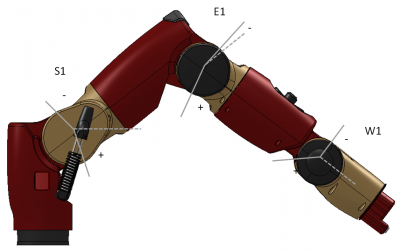
\includegraphics[height=\baselineskip]{imagenes/metodos/baxter_range_motion1.png}
%		\label{algo} \quad
%	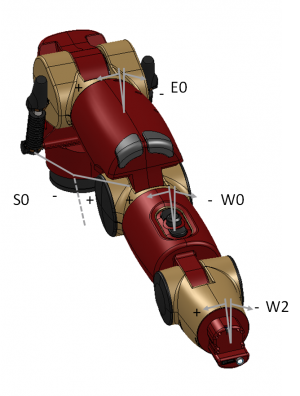
\includegraphics[height=\baselineskip]{imagenes/metodos/baxter_range_motion2.png}
%	\label{algo2}
%	}
%\end{center}
\begin{figure}[]
	\centering
	\begin{subfigure}[b]{0.4\textwidth}
		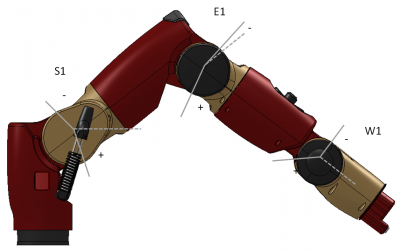
\includegraphics[trim=0 0 0 10, clip, width=\textwidth]{imagenes/metodos/baxter_range_motion1.png}
		\caption{Límites traslación}
		\label{fig:metodos/limits1}
	\end{subfigure}
	\begin{subfigure}[b]{0.4\textwidth}
		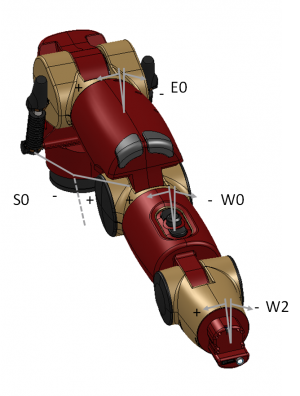
\includegraphics[width=\textwidth]{imagenes/metodos/baxter_range_motion2.png}
		\caption{Límites rotación}
		\label{fig:metodos/limits2}
	\end{subfigure}
	\caption{Límites articulaciones}
	\label{fig:metodos/limits}
\end{figure}
% Cambiar orden a pos, vel, torque, pos_raw

Dada la naturaleza del robot Baxter, en este modo de operación se aplican unos filtros antes de aplicar la orden de posición, a fin de evitar accidentes y otorgar una experiencia de movimiento más fluida y segura. Los filtros son los que se muestran en la figura \ref{fig:metodos/position_filters}.

\begin{figure}[]
	\centering
	\begin{subfigure}[b]{0.24\textwidth}
		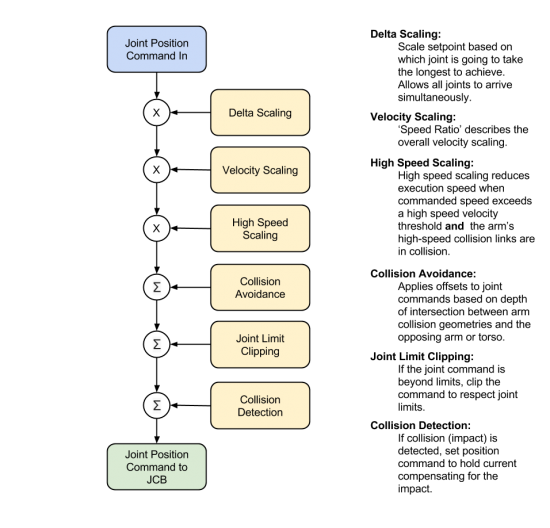
\includegraphics[trim=0 0 235 0, clip, width=\textwidth]{imagenes/metodos/baxter_position_filters.png}
		\caption{Control por posición}
		\label{fig:metodos/position_filters}
	\end{subfigure}
	\begin{subfigure}[b]{0.24\textwidth}
		\centering
		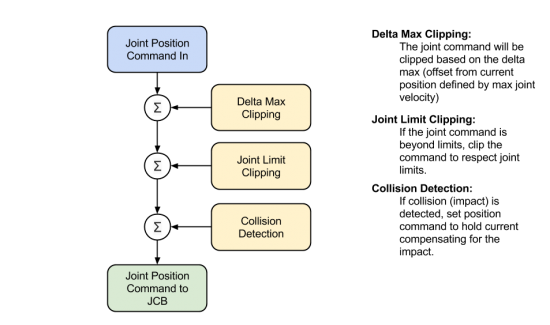
\includegraphics[trim=0 0 230 0, clip, width=\textwidth]{imagenes/metodos/baxter_position_raw_filters.png}
		\caption{Control por posición sin procesar}
		\label{fig:metodos/raw_filters}
	\end{subfigure}
	\begin{subfigure}[b]{0.24\textwidth}
		\centering
		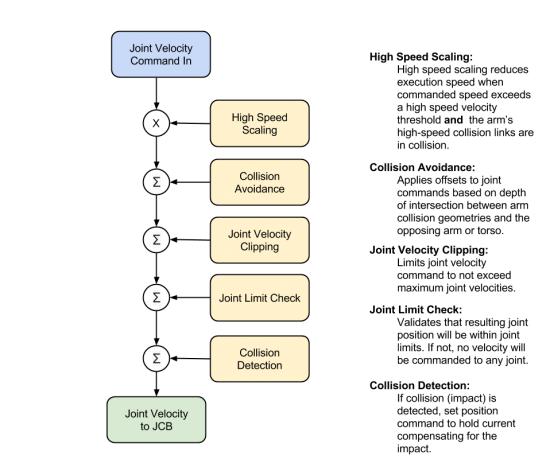
\includegraphics[trim=0 0 235 0, clip, width=\textwidth]{imagenes/metodos/baxter_velocity_filters.png}
		\caption{Control por velocidad}
		\label{fig:metodos/vel_filters}
	\end{subfigure}
	\begin{subfigure}[b]{0.24\textwidth}
		\centering
		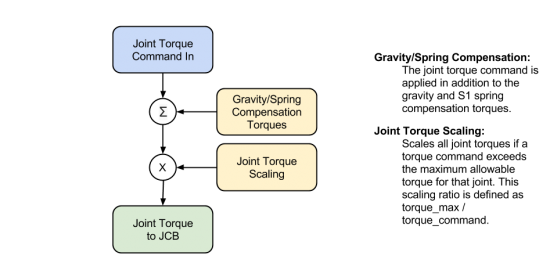
\includegraphics[trim=0 0 230 0, clip, width=\textwidth]{imagenes/metodos/baxter_torque_filters.png}
		\caption{Control por torque}
		\label{fig:metodos/torque_filters}
	\end{subfigure}
	\caption{Filtros aplicados}
\end{figure}

\begin{enumerate}
\item {Escalado delta.} Consiste en escalar las posiciones objetivo en el recorrido para conseguir que todas las articulaciones lleguen al punto deseado a la vez.
\item {Escalado de velocidad.} Se escala la velocidad de cada articulación en función del 'ratio de velocidad'.
\item {Escalado de alta velocidad.} Para evitar colisiones entre los dos brazos moviéndose el uno en la dirección del otro, se escala la velocidad y recalcula la posición cuando ésta supera un umbral.
\item {Prevención de colisiones.} Gracias a un modelo interno del robot, se limitan las posiciones de las articulaciones tales que provocarían un choque con el propio robot.
\item {Recorte de posiciones.} Si las posiciones superan los límites de la articulación, estas se recortan al límite permitido.
\item {Detección de colisión.} Si se detecta una colisión (con un objeto externo al robot), mantiene la última posición antes de la colisión.
\end{enumerate}

Como se puede observar, Baxter aplica unos filtros para evitar y detectar colisiones. Esta tarea se realiza de tres maneras:

\begin{itemize}
\item {Prevención.} El robot ejecuta una simulación interna, donde las articulaciones y el cuerpo cuentan con unas regiones de seguridad que, al tocarse, limitan el movimiento del robot.
\item {Detección de colisión.} Esto se realiza de dos maneras
\begin{enumerate}
\item [Impacto] Cuando el torque de cualquier articulación cambia bruscamente, se considera que ha habido una colisión.
\item [Retención] Cuando el torque aplicado aumenta pero la articulación no se mueve, se considera que está colisionando con un objeto inmóvil.
\end{enumerate} 
\item {Escalado de alta velocidad.} Cuando la velocidad del brazo supera los 0.2 m/s, las regiones de seguridad que el robot simula internamente aumentan. Cuando se tocan estas regiones, la velocidad se escala y la posición se recalcula.
\end{itemize}

\subsubsection{Control por posición sin procesar}
Este modo de control, al igual que el anterior, tiene como objetivo alcanzar la posición deseada para cada articulación. Se diferencia en los filtros que aplica (figura \ref{fig:metodos/raw_filters}).

\begin{enumerate}
\item {Recorte de delta máximo.} Recorta la posición siguiente (en el intervalo de actuación de cada articulación) a la máxima posición alcanzable a la velocidad máxima dada por la 'ratio de velocidad'.
\item {Recorte de posiciones.} Al igual que en el modo de control anterior, si las posiciones superan los límites de la articulación, estas se recortan al límite permitido.
\item {Detección de colisión.} Cumple la misma función que en el modo de control por posición.
\end{enumerate}

Como se puede observar, este es un modo de control más avanzado, ya que no tiene en cuenta las colisiones consigo mismo, y ofrece un movimiento más brusco al no llegar todas las articulaciones al punto destino a la vez.

El modo de control en el mensaje JointCommand es el 4.

\subsubsection{Control por velocidad}
En este modo de control, lo que se busca es adquirir la velocidad objetivo para cada articulación. El modo de control en el mensaje JointCommand es el 2. Al igual que en los modos anteriores, se aplican una serie de filtros (figura \ref{fig:metodos/vel_filters}).

\begin{enumerate}
\item {Escalado de alta velocidad.} Como en el control por posición.
\item {Prevención de colisiones.} Como en el control por posición.
\item {Recorte de velocidades.} Se limitan las velocidades para cada articulación para que no excedan el máximo permitido.
\item {Comprobación de límites.} Se comprueban los límites de las articulaciones. Si se exceden, se detiene el movimiento.
\item {Detección de colisión.} Igual que en el control por posición.
\end{enumerate}

El dejar de enviar velocidades si se exceden los límites de las articulaciones es una medida de seguridad que exige al programador tener el control sobre las posiciones que puede alcanzar el brazo.

\subsubsection{Control por torque}
El control por torque consiste en el modo de más bajo nivel que se puede controlar el robot Baxter. Los torques que enviemos serán aplicados por los controladores, haciendo uso solamente de los siguientes filtros (figura \ref{fig:metodos/torque_filters}):

\begin{enumerate}
\item {Compensación.} Los torques se suman a los necesarios para mantener la gravedad 0 y el muelle ubicado en la articulación s1 (traslación del hombro).
\item {Escalado de torque.} Si un torque excede el torque máximo para esa articulación, escala los torques de todas las articulaciones por el factor de exceso de esa articulación (torque\_max/torque).
\end{enumerate}

La compensación de la gravedad se puede desactivar mandando un mensaje vacío al tema \texttt{/robot\-/limb\-/right\-/suppress\_\-gravity\_\-compensation} para el brazo derecho, o \texttt{/robot\-/limb\-/left/\-suppress\_\-gravity\_\-compensation} para el brazo izquierdo.

De esta manera, un torque aplicado de 0 en todas las articulaciones, mantendrá el brazo en un estado de gravedad 0 si la compensación esta activa. De no estarlo, el brazo caerá en peso muerto.

\subsection{Simuladores}
\subsubsection{V-REP}
Virtual Robot Experimentation Platform (V-REP) \cite{vrep} es un simulador robótico muy potente, con una gran cantidad de modelos predefinidos listos para simular, y una gran cantidad de opciones para configurar.

\subsubsection{Gazebo}
Al igual que V-REP, Gazebo \cite{gazebo} es un simulador de plataformas robóticas. Es menos potente, y tiene menos modelos predefinidos, pero está integrado con \ros, y el robot Baxter cuenta con un modelo listo para simular para el mismo, por lo que es la opción elegida para realizar las pruebas.

\paragraph{Problemas}
La versión del simulador en la que está implementada es la 2.2, mientras que la que se puede descargar ahora es la 7.1. Esto hace que no sea lo potente que debiera, y a la hora de realizar simulaciones utilizando el control por torques, el simulador no responde igual que el robot, por lo que su uso quedó limitado a las primeras pruebas que se hicieron en una primera aproximación al control por posición del robot.

\section{Redes Neuronales}
Una red neuronal artificial \cite{abu2012learning} \cite{hinton} \cite{andrewng} es un conjunto de algoritmos de aprendizaje automático capaces de extraer modelos a partir de un conjunto de datos de aprendizaje. De esta manera, estos sistemas son capaces de emular la fuente generadora de datos y producir salidas coherentes a partir de entradas no vistas con anterioridad.
\subsection{Topología}
En función de la topología de la red, se contemplan dos tipos fundamentales: las redes hacia adelante, y las redes recursivas. A continuación se habla de las redes hacia delante, mientras que las redes recursivas se analizan en un apartado más adelante.
\subsubsection{Redes hacia adelante}
Las conexiones entre las neuronas es de un solo sentido, de modo que no se forman bucles entre ninguna de las neuronas (figura \ref{fig:metodos/feedforward}). Las líneas que conectan las ``neuronas'' son pesos, y la interconexión entre una capa y otra se puede representar como una matriz de mxn, donde m es el número de neuronas de la capa anterior, y n es el numero de neuronas de la capa siguiente. De este modo, la entrada de cada capa no es sino la combinación lineal de las salidas de las capas anteriores.

Si las relaciones entre las capas sólo fueran combinaciones lineales, la red neuronal se podría reducir a una única matriz que interconectara la capa de entrada con la de salida. Lo que sucede es que cada neurona tiene una activación, que consistirá en una relación no lineal entre la entrada que percibe y la salida. Son estas no linealidades las que le confieren la capacidad de aprender parámetros nuevos, por lo que podrán ajustarse al espacio de búsqueda.

\begin{figure}
	\centering
	\begin{subfigure}[b]{0.5\textwidth}
		\centering
		\begin{neuralnetwork}[height=4.7]
			\newcommand{\nodetextclear}[2]{}
			\newcommand{\nodetextx}[2]{$x_#2$}
			\newcommand{\nodetexty}[2]{$y_#2$}
			\newcommand{\nodetexth}[2]{$h_{#1#2}$}
			\inputlayer[count=4, bias=false, title=Capa de\\entrada, text=\nodetextx]
			\hiddenlayer[count=5, bias=false, title=Capa\\oculta, text=\nodetexth] \linklayers
			\outputlayer[count=3, title=Capa de\\salida, text=\nodetexty] \linklayers
		\end{neuralnetwork}
		\caption{Red monocapa}
		\label{fig:metodos/feedforward1}
	\end{subfigure}
	\begin{subfigure}[b]{0.49\textwidth}
		\centering
		\begin{neuralnetwork}[height=4.7]
			\newcommand{\nodetextclear}[2]{}
			\newcommand{\nodetextx}[2]{$x_#2$}
			\newcommand{\nodetexty}[2]{$y_#2$}
			\newcommand{\nodetexth}[2]{$h_{#1#2}$}
			\inputlayer[count=4, bias=false, title=Capa de\\entrada, text=\nodetextx]
			\hiddenlayer[count=5, bias=false, title=Capa\\oculta, text=\nodetexth] \linklayers
			\hiddenlayer[count=5, bias=false, title=Capa\\oculta, text=\nodetexth] \linklayers
			\outputlayer[count=3, title=Capa de\\salida, text=\nodetexty] \linklayers
		\end{neuralnetwork}
		\caption{Red multicapa}
		\label{fig:metodos/feedforward2}
	\end{subfigure}
	\caption{Redes neuronales de propagación hacia adelante}
	\label{fig:metodos/feedforward}
\end{figure}

\paragraph{Activaciones}
Las activaciones más usadas son las siguientes.
\subparagraph{Sigmoidea}
Consiste en una función cuyo rango va de 0 a 1. Esto permite interpretar su salida como una probabilidad. Es muy usada en tareas de clasificación (figura \ref{fig:metodos/sigmoid}).
\subparagraph{Sigmoidea ``dura''}
Se trata de una aproximación de la función sigmoidea a trozos, tal y como se muestra en la figura \ref{fig:metodos/hard-sigmoid}.
\subparagraph{Tangente hiperbólica}
Tiene un comportamiento parecido a la sigmoidea, pero su rango va de -1 a 1, y es simétrica. (figura \ref{fig:metodos/tanh}).
	
\subparagraph{Rectificador lineal (ReLU)}
Se trata de la función lineal rectificada. Es muy usada en redes neuronales profundas (explicadas más adelante) debido a las características de la derivada (figura \ref{fig:metodos/relu}).

\paragraph{Errores}
Para calcular el rendimiento de una red se utilizan los errores a la salida, que consiste en aplicar una función a los valores obtenidos y los deseados. Las funciones más comunes son las siguientes:

\subparagraph{MAE}
El error absoluto medio (MAE) es la media del valor absoluto de la diferencia de los errores cometidos en cada neurona a la salida. Usado en problemas de regresión lineal (la salida es una curva función de los datos de entrada).
\subparagraph{MSE}
El error cuadrático medio (Mean Squared Error) consiste en la media de los cuadrados de la diferencia de los errores cometidos en cada neurona a la salida. Se utiliza también en regresión lineal.
\subparagraph{Entropía cruzada}
Su fórmula es $H(p, q) = -\sum_{x}{p(x)\log q(x)}$ y es usada en tareas de clasificación, ya que da un mayor sentido a la probabilidad que representa la salida de este tipo de redes.

\begin{figure}
	\begin{subfigure}[b]{0.5\textwidth}
		\centering
		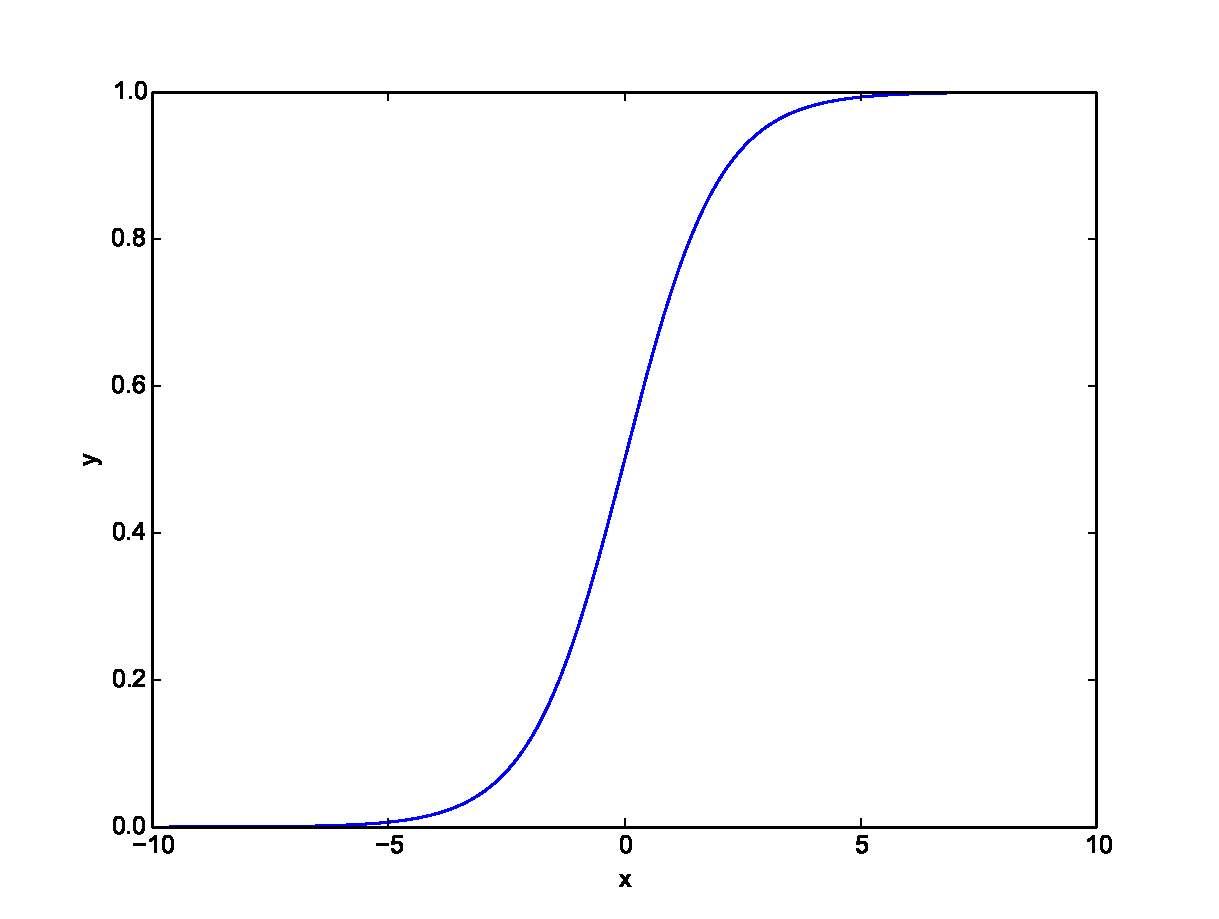
\includegraphics[width=\linewidth]{imagenes/metodos/sigmoid.pdf}
		\caption{Función sigmoidea}
		\label{fig:metodos/sigmoid}
	\end{subfigure}
	\begin{subfigure}[b]{0.5\textwidth}
		\centering
		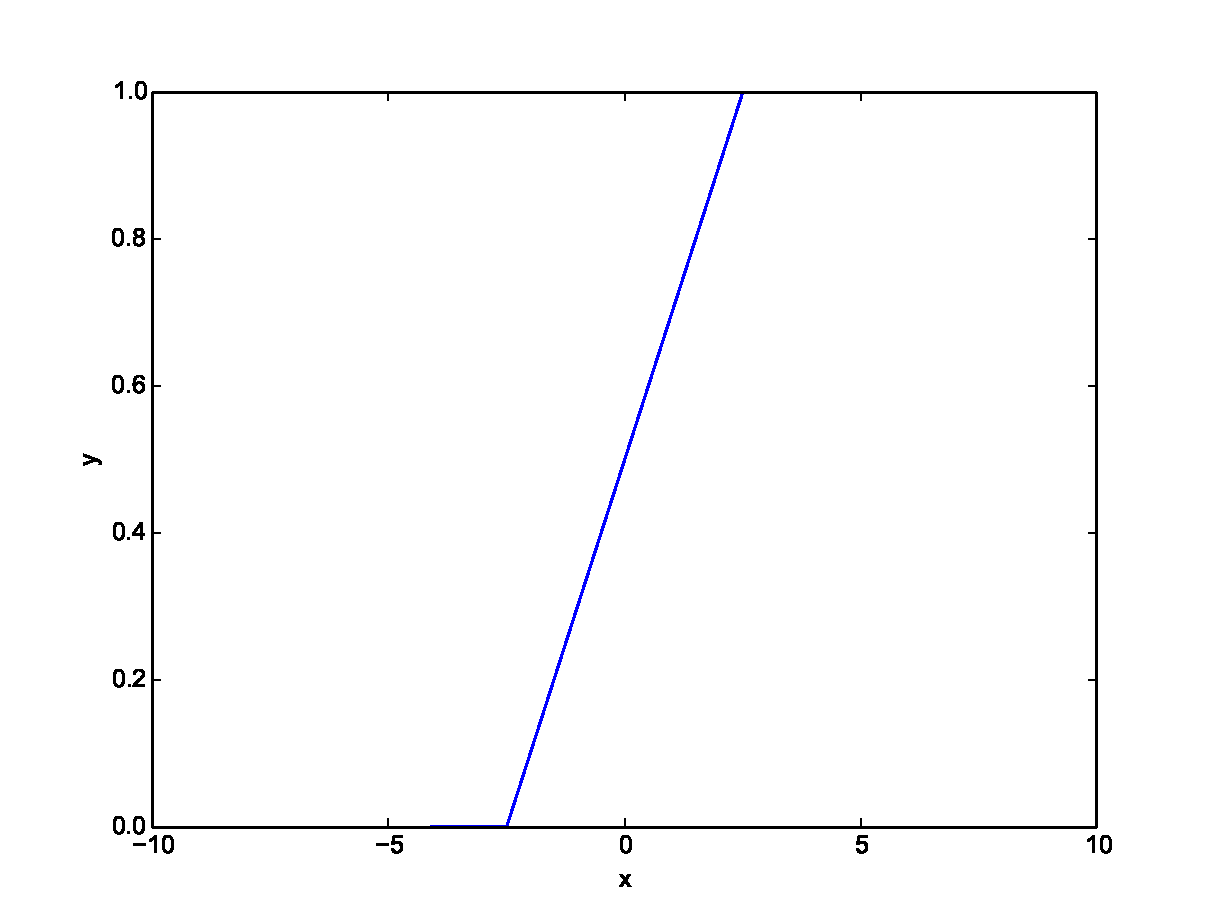
\includegraphics[width=\linewidth]{imagenes/metodos/hard-sigmoid.pdf}
		\caption{Función sigmoidea ``dura''}
		\label{fig:metodos/hard-sigmoid}
	\end{subfigure}
	\begin{subfigure}[b]{0.5\textwidth}
		\centering
		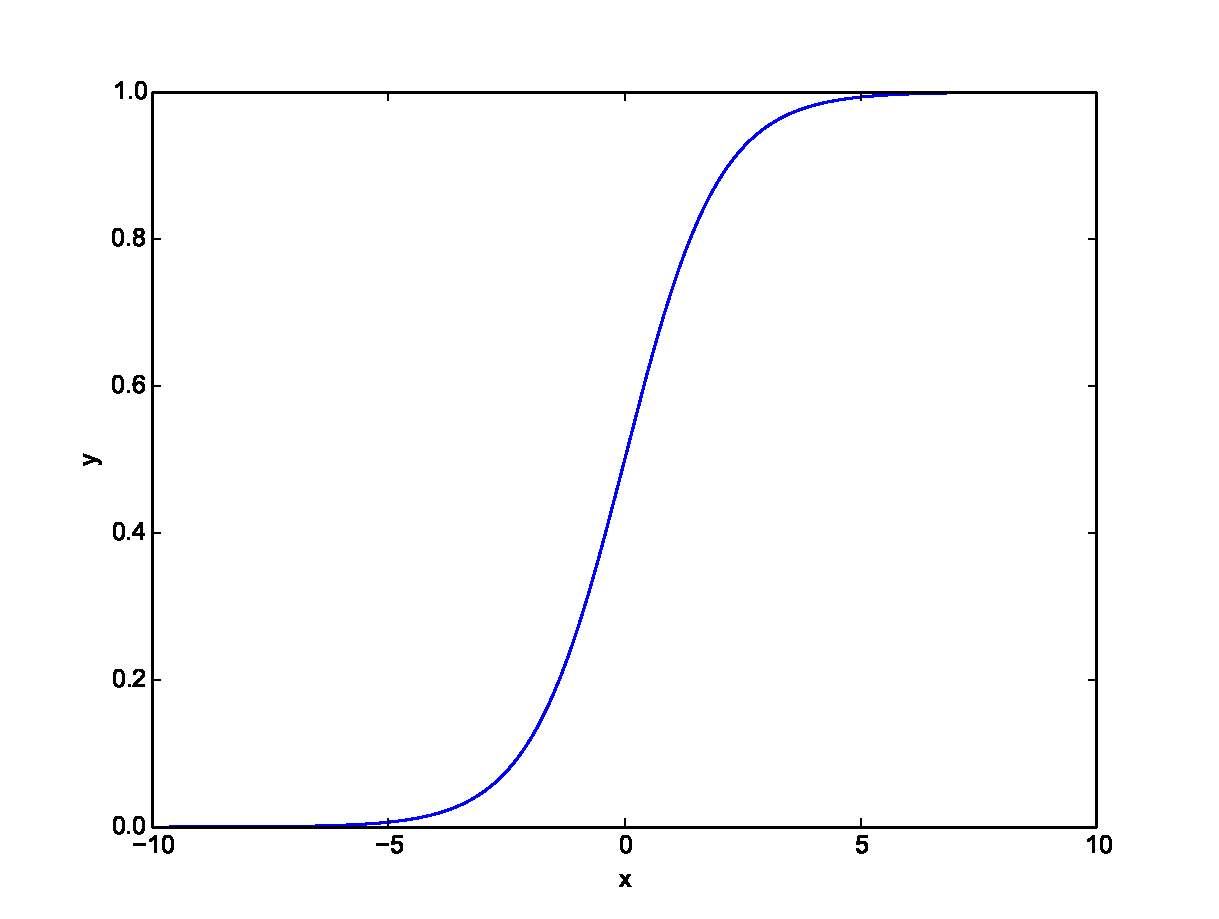
\includegraphics[width=\linewidth]{imagenes/metodos/sigmoid.pdf}
		\caption{Tangente hiperbólica}
		\label{fig:metodos/tanh}
	\end{subfigure}
	\begin{subfigure}[b]{0.5\textwidth}
		\centering
		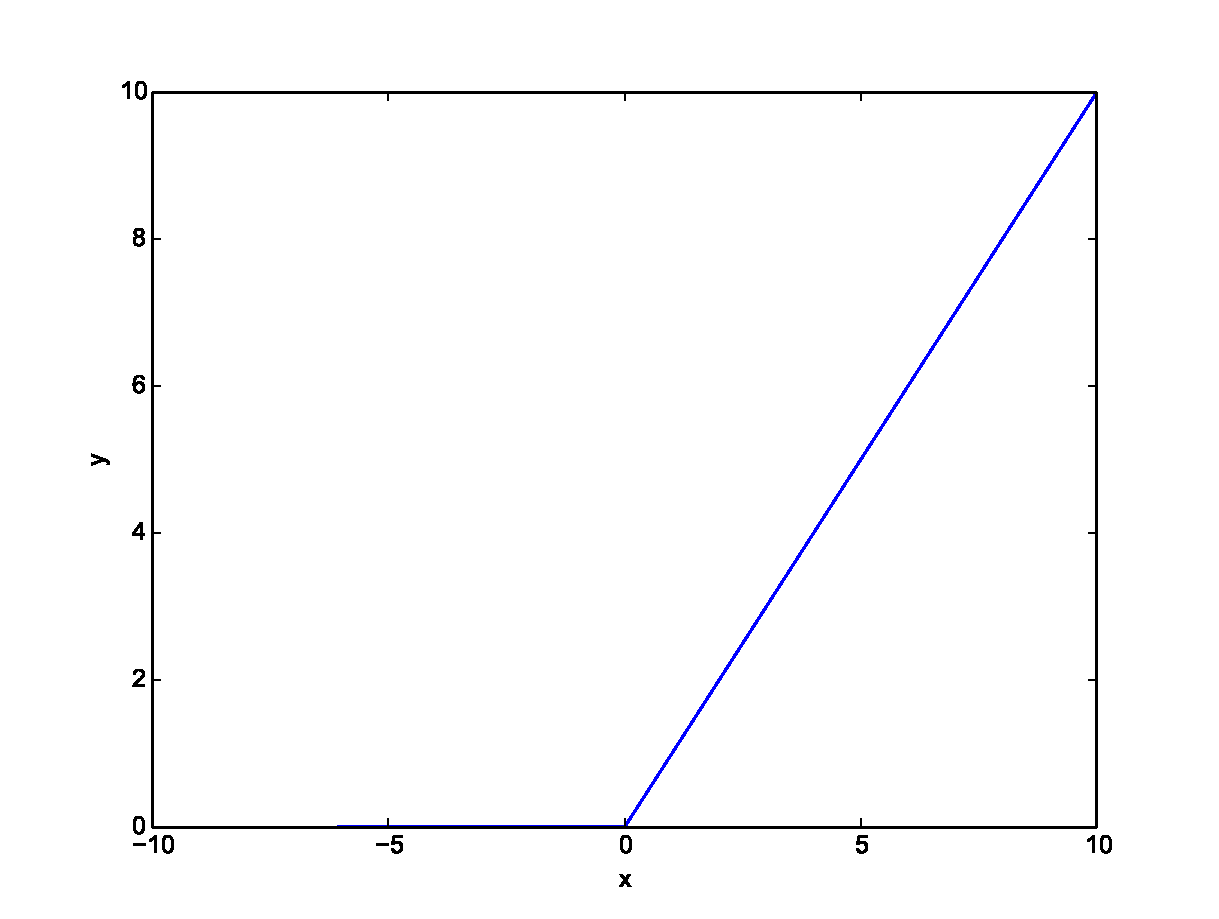
\includegraphics[width=\linewidth]{imagenes/metodos/relu.pdf}
		\caption{Rectificador lineal}
		\label{fig:metodos/relu}
	\end{subfigure}
	\caption{Activaciones}
	\label{fig:metodos/activations}
\end{figure}
\paragraph{Perceptron}
Fue el primer tipo de red neuronal. La manera de obtener las salidas es igual a la explicada anteriormente.

El entrenamiento de este tipo de red neuronal consiste en minimizar el error de los pesos (relaciones entre las neuronas). Esto significa que, suponiendo que hay un conjunto de pesos que permite obtener la salida correcta para cada una de las entradas, el perceptrón iterará sobre cada uno de los pesos hasta encontrar un subconjunto de estos pesos.

El problema radica en que puede no existir dicho conjunto, y por lo tanto el perceptrón no será capaz de encontrar los pesos.

Es por esto por lo que su uso queda restringido a problemas donde las características sean separables.

\paragraph{Propagación hacia atrás de errores}
Otra manera de entrenar la red, consisten en encontrar el conjunto de pesos que minimiza una función error, generada por los errores cometidos a la salida de la red.

Al contrario que en el perceptrón, esta tipo de entrenamiento permite encontrar un mínimo local en el espacio de los pesos para el conjunto de datos, aunque estos no sean separables.

El algoritmo de actualización de los pesos usado es el de propagación hacia atrás de errores. Consiste en, a partir del error generado en la salida, se reduce cada uno de los pesos en función de la cantidad de error asociado a dicho peso. Para realizar este algoritmo, se requiere de las derivadas de los errores cometidos en cada neurona, a fin de obtener la relación entre el error final del que cada neurona es responsable.

Hay distintos tipos de algoritmos \cite{gradient_descent} que implementan la propagación hacia atrás de errores.

\subparagraph{Descenso en gradiente}
Consiste en el algoritmo más sencillo. Dada la relación entre el error total y el generado por cada peso, modifica el peso de manera proporcional a dicho error. Esto, visto en el espacio de los pesos con respecto al error total, significa descender por la curva en la dirección y sentido de mayor pendiente (de ahí el nombre).
\subparagraph{Descenso en gradiente estocástico}
Es como el anterior, pero, en vez de calcular el error para todo el conjunto de datos de entrenamiento, se calcula el error en pequeños grupos y se aplica el algoritmo. Esto produce que el descenso no se produzca en la dirección de máxima pendiente del conjunto, sino del subconjunto. El método funciona porque la media de dichos descensos aproxima el descenso total. Al caso en el que el subconjunto es una sola muestra se le llama aprendizaje online.
\subparagraph{Momentum}
Es una modificación al descenso en gradiente, en el que la dirección de descenso se ve alterada por los descensos producidos en iteraciones anteriores. Esto le da la característica de ``velocidad'' al punto de operación.
\subparagraph{Adam}
La estimación adaptativa del momento hace uso de la técnica del momento, y adapta la cantidad de descenso en gradiente para cada uno de los parámetros a optimizar, de modo que, los parámetros cuyo rango de operación es más pequeño perciben cambios más pequeños en la actualización de su valor.

\subsubsection{Redes recursivas}
\label{subsubsec:metodos/recursivas}
Las redes recursivas \cite{karpathy} son el otro tipo de redes en función de la topología de la red, y difieren de las redes hacia delante en que las neuronas pueden conectarse entre sí hacia atrás (o consigo mismas), generando en la red una realimentación entre nodos que provoca que la salida de la red no dependa sólo de la entrada, sino del estado de la misma (que varía en función de su historia) (fig. \ref{fig:metodos/rnn}).

Tienen la capacidad de aprender de sistemas cuyo comportamiento cambia con el tiempo.
\begin{figure}
	\centering
	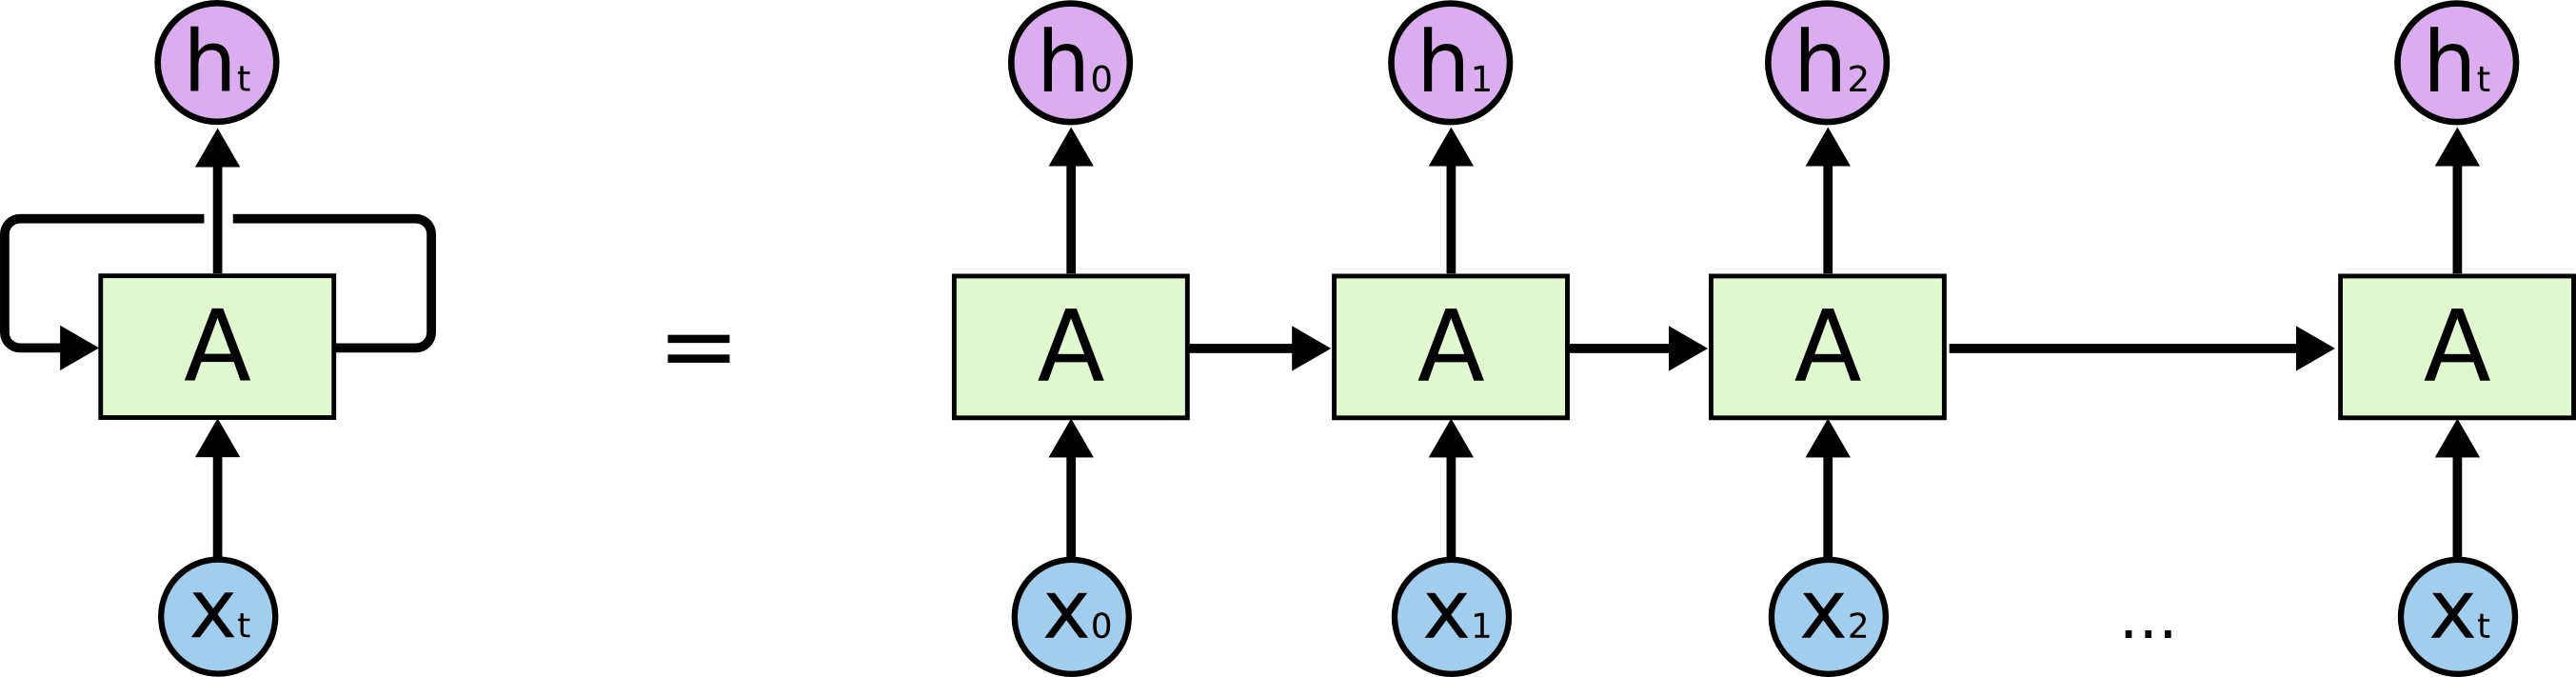
\includegraphics[height=3cm]{imagenes/metodos/rnn.png}
	\caption{Red neuronal recurrente [Fuente: \cite{colah}]}
	\label{fig:metodos/rnn}
\end{figure}
\paragraph{Redes recurrentes}
Es el tipo de red recursiva más básica. Consiste en un conjunto de neuronas (normalmente agrupados en una capa) cuya salida no depende solamente de las entradas provenientes de capas anteriores, sino que también dependen de las salidas de las neuronas en esa misma capa. De esta manera, el estado de la red cambia conforme cambian las salidas de esta capa.
\paragraph{LSTM}
Las redes de memoria a corto y largo plazo (Long Short Term Memory) \cite{hochreiter1997long}\cite{colah} hacen uso de una unidad especial, que consiste en un conjunto de puertas que permiten el flujo de información a través de la neurona. En concreto, cuenta con 3 puertas:

\begin{itemize}
	\item Puerta de entrada. Su valor varía de 0 a 1 y se multiplica al valor de la entrada de la activación.
	\item Puerta de salida. Igualmente, su valor varía de 0 a 1 y se multiplica al valor de la salida después de la activación.
	\item Puerta de olvido. Representa la cantidad del estado anterior que se mantiene.
\end{itemize}

Todas estas puertas son activaciones sigmoideas que se activan con las entradas de la celda y con el estado de la misma.
\paragraph{GRU}
Las celdas GRU (Gated Recurrent Unit) \cite{chung2014empirical} son, al igual que las LSTM, celdas que hacen uso de puertas. Son más sencillas que las anteriores, y requieren menos cómputo, por lo que son más rápidas de entrenar. Cuentan con dos puertas en vez de tres: reinicio y actualización (fig. \ref{fig:metodos/gru})

La salida es una interpolación lineal del estado anterior y el nuevo estado propuesto, el cual se calcula como una combinación de la entrada y el estado anterior (multiplicado por la puerta de reinicio). La puerta de actualización se calcula a partir del estado anterior y la entrada, al igual que la puerta de reinicio.

\begin{figure}
	\begin{subfigure}[b]{0.5\textwidth}
		\centering
		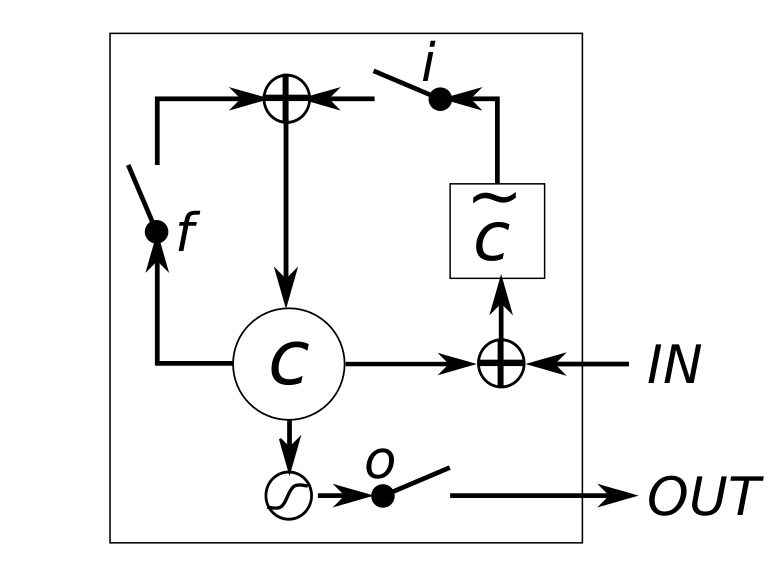
\includegraphics[width=\linewidth]{imagenes/metodos/lstm.png}
		\caption{Celda LSTM [Fuente: \cite{chung2014empirical}]}
		\label{fig:metodos/lstm}
	\end{subfigure}
	\begin{subfigure}[b]{0.5\textwidth}
		\centering
		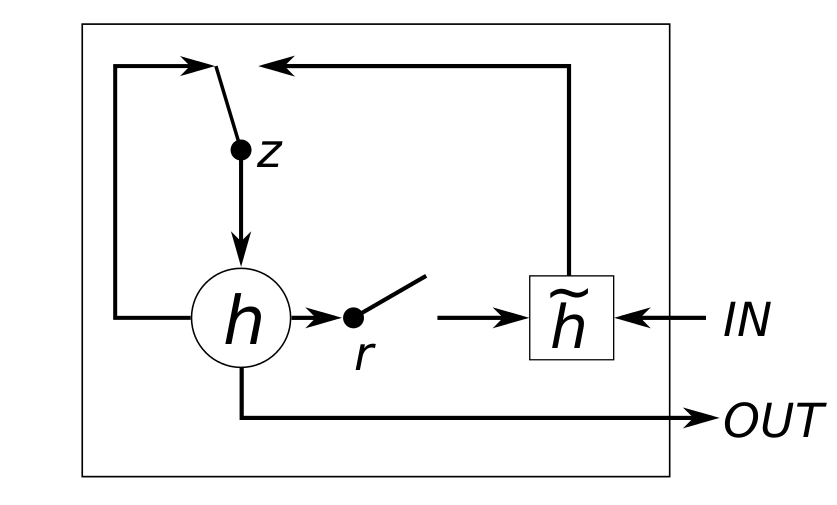
\includegraphics[width=\linewidth]{imagenes/metodos/gru.png}
		\caption{Celda GRU. [Fuente: \cite{chung2014empirical}]}
		\label{fig:metodos/gru}
	\end{subfigure}
\end{figure}
\paragraph{Propagación hacia atrás de errores en el tiempo}
El algoritmo de optimización de parámetros en el tiempo es el mismo usado en las redes hacia delante (propagación hacia atrás de errores), con la peculiaridad de que la red se desenrolla en el tiempo. Esto significa, que las neuronas realimentadas se interconectan entre sí en cada instante temporal (desenrollado). Las pérdidas se calculan de la misma manera, calculando el error en cada instante temporal (si es que se tiene una salida en cada instante) y aplicando el algoritmo de propagación hacia atrás sobre cada neurona.

Esta es la principal razón por la que surgieron las celdas LSTM y GRU, ya que, haciendo uso nada más de las redes recurrentes, se tiene el problema de desvanecimiento y explotación de los pesos de la red \cite{bengio1994learning}. Este fenómeno surge cuando la red se desdobla un número lo suficientemente grande como para que, al propagar hacia atrás el error, debido a la gran dimensionalidad de la red, el error llegue muy reducido (desvanecimiento) o muy amplificado (explotación), impidiendo que, alcanzado este punto, la red aprenda.

\subsection{Regularización}
Las redes neuronales son sistema capaces de aprender a extraer patrones de los datos que se le ofrecen. Por lo tanto, se podría pensar que una red lo suficientemente grande es capaz de extraer cualquier patrón que haya en los datos. Esto es ideal si contamos con una base de datos infinita, ya que cualquier discrepancia entre muestras se tomaría como ruido y la red no aprendería de éste. El problema es que no se puede aprender de una base de datos infinita (el tiempo de cálculo sería igualmente infinito), y no se puede obtener dicha base de datos.

Una vez asumido que no se puede disponer de esta base de datos, nos encontramos con el problema de que, en una base finita, podemos no tener representados todos los casos de estudio que nos interesan, esto es, que la base de datos no sea representativa de la realidad de la que se pretende aprender. En este caso, lo mejor que puede hacer la red es aprender de dichas muestras, y sería incapaz de generalizar para el conjunto no visto (o no visto lo suficiente).

También nos encontramos con que cada muestra por sí misma puede contener ruido (de los sensores, de un error en el proceso de obtención...). En este caso, si no se toman medidas, la red aprenderá también estos patrones, lo que reducirá aumentará el error cuando se enfrente a muestras que no ha visto antes (y sobre las que el ruido ha influido de manera distinta).

Es por esto, por lo que se requieren de técnicas de regularización, para evitar el sobreentrenamiento de la red (overfitting). Algunas de estas técnicas son las siguientes.

\subsubsection{Infradimensionamiento de la red}
La primera medida que se puede tomar es ajustar el tamaño de la red al problema que se esté abarcando. De esta manera, se elimina el problema de base de que las redes más grandes son las que mejor encuentran patrones (en este caso de estudio, de ruido).
\subsubsection{L2}
El problema del sobredimensionamiento es que las neuronas se especializan demasiado (capaces de reconocer el ruido). Esta especialización se da debido a que algunos pesos de interconexión de neuronas se vuelven muy altos, eliminando la influencia que tienen el resto de entradas en una misma neurona.

Una solución a este problema es añadir un error proporcional al cuadrado de los pesos de cada neurona (error L2). De esta manera, los pesos altos (especializados) aumentarán el error, y en el paso de propagación hacia atrás de errores se reducirá dicho peso.
\subsubsection{L1}
La regularización L1, al igual que la L2 \cite{ng2004feature}, consiste en la aportación de los pesos al error, pero a diferencia de ésta, esta aportación es lineal proporcional (no cuadrática). Esto ayuda a seleccionar un conjunto de neuronas, que se especializarán, pero, al ser un número reducido de ellas, esta especialización promoverá el aprendizaje de los patrones más importantes de los datos de entrenamiento, y por lo tanto, la eliminación del ruido.
\subsubsection{Dropout}
Dropout \cite{gal2015theoretically} es una técnica de regularización que se basa en el hecho de que, la media ponderada de un conjunto de redes neuronales, cada una especializada en un subconjunto de datos, genera unos resultados mejores que cada una de las redes individualmente. Esto se debe a que cada red puede haber adquirido un error distinto, pero al juntarlas, este error disminuye.

El problema es que entrenar redes neuronales es un proceso computacionalmente costoso. Es por esto por lo que esta técnica propone realizar dicha media en la fase de entrenamiento. Para ello, en la fase de propagación hacia adelante, anula cada neurona con una probabilidad $p$, de modo que la salida va a depender de una subconjunto de las neuronas de la red (entre las cuales pueden estar o no las neuronas especializadas). De esta manera, se consigue que las dependencias con las neuronas más especializadas se reparta sobre varias neuronas, de modo que se reduce el error, al depender de varias neuronas, cada una con su versión reducida del error.
\subsection{Aprendizaje profundo}
Aprendizaje profundo (Deep Learning) \cite{schmidhuber2015deep}\cite{udacitydeeplearning} es un conjunto de técnicas usadas sobre las redes neuronales que le permiten alcanzar resultados nunca antes conseguidos en el campo del aprendizaje automático.

En un sentido amplio, el aprendizaje profundo consiste en una red neuronal con un gran número de capas y un gran número de neuronas por capas. Esto le da la capacidad de abarcar cualquier problema, pero también tiene el problema de que la red, de no tomar las medidas adecuadas, aprenderá incluso el error que hay en la base de datos de entrenamiento (overfitting).

Este error se disminuye haciendo uso de la técnica de regularización dropout, utilizado en conjunción con el error L2 y/o el error L1.

Este tipo de redes son realmente potentes cuando se entrenan con grande bases de datos de entrenamiento. El problema de estas bases de datos, es que para realizar el algoritmo de propagación hacia atrás de errores, es necesario calcular el error de cada neurona, y para ello hay que calcular la derivada y la aportación de cada neurona al error. Esto supone una gran cantidad de recursos (tanto de procesamiento, realizado en GPU, como de memoria) que en ocasiones no se puede abarcar. Para solucionar este problema, se utilizan algoritmos de propagación hacia atrás de errores basados en la división de la base de entrenamiento en grupos (descenso en gradiente estocástico).

Como se ha comentado, hay que calcular las derivadas para conocer la aportación de cada neurona al error. Esto supone un gran coste computacional, por lo que se utilizan funciones no lineales con derivadas fáciles de calcular, como las activaciones relu o la sigmoide ``dura''.

\subsection{Evaluación}
Para evaluar el rendimiento de la red neuronal, se divide la base de datos en dos conjuntos, uno de entrenamiento y otro de test. El primero servirá para entrenar la red, cada uno de los pesos. El segundo servirá para calcular el error que comete esa red sobre un conjunto de datos no vistos en el entrenamiento.

Además, se puede dividir los datos en un tercer conjunto, llamado de validación \cite{kohavi1995study}, para ajustar parámetros de la red, como número de neuronas por capa, número de capas, proporción usada en dropout, en L1, L2, distintas topologías... El motivo por el que no se puede usar el conjunto de test para este fin y ha de utilizarse uno distinto, es debido a que este conjunto lo vamos a utilizar para tomar decisiones sobre la red basadas en el rendimiento que se obtiene con dicho conjunto. Es por esto, por lo que el error obtenido en el conjunto de test (de usarse como de validación) no sería válido, ya que la red ha sido diseñada para adaptarse a dicho conjunto, y por lo tanto, a la hora de enfrentarse a datos nuevos, no desempeñaría con la eficacia esperada.

\subsection{Herramientas}
Diseñar los algoritmos mencionados no es tarea fácil, y mucho menos hacerlo con la eficiencia que se necesita para que estas técnicas sean viables. Es por esto por lo que existen diversas plataformas de diseño de redes neuronales, con los algoritmos de propagación hacia atrás de errores, las topologías, activaciones y métodos de regularización ya implementadas.

Entre ellas se encuentran \textit{Theano}, \textit{Tensorflow} \cite{tensorflow}, \textit{Caffe} \cite{caffe}, \textit{Torch} \cite{torch}... Además, contamos con librerías que, sobre estas anteriores, ofrecen una capa de abstracción para diseñar y entrenar redes neuronales profundas, como Keras \cite{keras} y Lasagne \cite{lasagne}.

Las librerías usadas en este trabajo son \textit{Tensorflow} y \textit{Keras}, debido a que están escritos en Python (facilitando la integración con la API de Baxter, así como \textit{rospy}) y que cuentan con una gran comunidad detrás que hace sencillo su aprendizaje y la resolución de problemas que van surgiendo conforme se va desarrollando.
\subsubsection{Tensorflow}
Creada por Google, esta librería se basa en la descripción de la red mediante variables simbólicas. El conjunto de estas variables y las relaciones entre ellas se denominan gráficos. Una vez creados los gráficos, se ejecutan en el contexto de sesiones, ofreciendo así una forma de abstracción con respecto a lo que sucede en los gráficos. Estas sesiones pueden ejecutarse en CPUs, o más eficientemente, en GPUs.

Las gráficas se forman relacionando nodos mediante operaciones con tensores. Un tensor es un vector n-dimensional. Los nodos pueden ser de entrada, constantes, variables, o módulos que implementan operaciones más complejas ya creados, como \texttt{matmul} (multiplicación de tensores), o \texttt{Gradient\-Descent\-Optimizer}.

A continuación, la gráfica se carga en una sesión, se le ofrecen los valores que necesita (entradas, valores auxiliares) y se le piden los nodos que se necesitan (el de entrenamiento, para que ejecute un paso de descenso en gradiente). Las gráficas, al igual que los datos necesarios para su ejecución, se cargan completamente en la CPU/GPU, de modo que no son necesarias hacer llamadas al sistema para adquirir los recursos, haciendo la computación mucho más rápido.
\paragraph{Tensorboard}
Dentro de \textit{tensorflow} tenemos la utilidad \textit{tensorboard}, que es una herramienta para visualizar el entrenamiento. En ella se puede monitorizar el error de la red en función del tiempo, así como la distribución de los pesos en cada una de las capas. Es una herramienta útil para saber si la red sufre de overfitting y las razones por las que lo hace.

\subsubsection{Keras}
\textit{Keras} por su parte, es una librería que ofrece al desarrollador una serie de funciones que permiten la abstracción de las operaciones que se ejecutan por debajo (sobre \textit{tensorflow} o \textit{theano}). Está creada especialmente para diseñar redes profundas. Cuenta con módulos como \texttt{Dense}, que no es más que una capa totalmente conectada con la siguiente, así como \texttt{GRU}, que implementa una capa formada por celdas GRU. También incluye los métodos de regularización explicados anteriormente, así como las activaciones.

Se usa diseñando la red en el entorno de un modelo. Tiene dos manera de crearla: secuencial, y utilizando directamente los modelos. La primera permite crear de manera sencilla una red donde cada capa se conecta con la siguiente, con una capa de entrada y otra de salida. La segunda permite configuraciones más complejas, como dividir la red en varias subredes, aceptar distintas entradas, y distintas salidas.

Una vez generado el modelo, sólo hace falta compilarlo (diciéndole qué algoritmo queremos usar para la fase de optimización, así como el tipo de error usado) y ejecutar la orden \texttt{fit}, que realiza una iteración sobre todo el conjunto de entrenamiento que le hayamos dado. Esta orden permite especificar el tamaño del grupo usado para realizar cada paso en la optimización (descenso en gradiente estocástico).
\section{Controladores}
Los controladores \cite{kulakowski2007dynamic}\cite{brosilow2002techniques}\cite{tolu2013adaptive}\cite{tolu2012bio} son sistemas que modifican un estado del que no se tiene directamente control en función de una señal de entrada. Esta modificación la hacen a través de señales que se envían a los actuadores, que sí que tienen la capacidad de cambiar el estado.

A la señal que nos indica el estado deseado se le llama señal de referencia, mientras que a la generada por el controlador se le llama de control. A la 

Ejemplos de controladores son los usados en regulación de la temperatura, donde no se tiene control sobre la misma directamente, sino que a lo que se tiene acceso es al voltaje aplicado a la fuente generadora de calor. Otro ejemplo es el control de velocidad de un motor. El motor es el actuador, y se le puede aplicar más o menos voltaje, en función del cual aplica el motor va más o menos rápido. A este motor se le anexiona una rueda, con lo que el motor ahora se encuentra con una fuerza que se opone a la dirección del movimiento, provocando que la velocidad del motor baje a un mismo voltaje.

Es a este tipo de problemas a los que los controladores se enfrentan y a los que deben ofrecer una solución.

\subsection{Error distal}
El error distal hace referencia a la diferencia entre el estado deseado y el estado actual. El nombre hace referencia a que no es un error que dependa directamente del controlador.
\subsection{Control realimentado}
Un sistema de control se dice que es realimentado si la señal de control que ofrece depende del estado actual. La salida del sistema será función del estado deseado y del estado actual. En concreto, este tipo de sistemas son función del error distal, y no tienen en cuenta los valores concretos de los estados deseados y actuales. En la figura \ref{fig:metodos/feedback_control} se puede observar el diagrama de bloques de este tipo de sistemas.

Un problema al que se hace frente en el diseño de controladores realimentados (como en cualquier sistema que lo sea), es la estabilidad del sistema. Es por esto por lo que se hay que estudiar que se cumpla dicha estabilidad en el diseño y uso de este tipo de sistemas.

\begin{figure}[]
	\centering
	\deactivatequoting
	\begin{tikzpicture}[auto, node distance=2cm,>=latex']
	% We start by placing the blocks
	\node [input, name=input] {};
	\node [sum, right of=input] (sum) {};
	\node [block, right of=sum] (controller) {Controlador\\realimentado};
	\node [block, right of=controller, node distance=3cm] (actuador) {Actuador};
	\node [block, right of=actuador, node distance=3cm] (system) {Sistema};
	% We draw an edge between the controller and system block to 
	% calculate the coordinate u. We need it to place the measurement block. 
	\node [output, right of=system] (output) {};
	\node [block, below of=actuador] (measurements) {Medidas};
	\node [block2, above of=system] (perturbacion) {Perturbación};
	
	% Once the nodes are placed, connecting them is easy. 
	\draw [draw,->] (input) -- node[name=inp] {$r(t)$} (sum);
	\draw [->] (sum) -- node {$e(t)$} (controller);
	\draw [->] (controller) -- node[name=c] {$c(t)$} (actuador);
	\draw [->] (actuador) -- node[name=u] {$u(t)$} (system);
	\draw [->] (system) -- node [name=y] {$y(t)$}(output);
	\draw [->] (y) |- (measurements);
	\draw [->] (perturbacion) -- (system);
	\draw [->] (measurements) -| node[pos=0.95] {$-$}
	node [near end] {$y_m(t)$} (sum);
	\end{tikzpicture}
	\caption{Sistema de control realimentado}
	\label{fig:metodos/feedback_control}
	\activatequoting
\end{figure}

\subsubsection{Controlador PID}
El controlador PID \cite{rivera1986internal} es un controlador lineal realimentado ampliamente usado en sistemas de control (fig. \ref{fig:metodos/pid_control}).

Se caracteriza por ser la suma de tres componentes de la señal de entrada: una parte proporcional a esta, una parte de la derivada, y otra de la integral. De este modo, tenemos tres controladores en uno. El sistema total es la suma ponderada de cada una de estos controladores.


\paragraph{Controlador P}
Es el controlador más sencillo. Consiste en aumentar la señal de control conforme aumenta la señal de error, e igualmente, disminuirla cuando la señal de error lo hace. De esta manera, aproximamos el estado actual al deseado y disminuimos el error.

\paragraph{Controlador I}
Este controlador hace uso de la parte integral de la señal. Para ello, se tiene en cuenta la historia del sistema y se realiza una acumulación ponderada de la historia del mismo. Este controlador sirve para ajustar el error constante que puede haber entre el estado deseado y el actual dada la señal de control generada por el controlador P, una vez que este se estabiliza.

\paragraph{Controlador D}
El controlador D consiste en cambiar la señal de control proporcionalmente a la derivada de la señal de error. De esta manera, si el controlador P está acercando rápidamente el estado actual al deseado (disminuyendo así el error), este controlador generará una señal de sentido contrario a la generada por el controlador P, con el fin de disminuir las oscilaciones producidas por este cuando alcanza la posición deseada a gran velocidad. 

\begin{figure}[]
	\centering
	\deactivatequoting
	\begin{tikzpicture}[auto, node distance=2cm,>=latex']
	% We start by placing the blocks
	\node [input, name=input] {};
	\node [block, right of=input] (controllerp) {Controlador P};
	\node [block, above of=controllerp] (controllerd) {Controlador D};
	\node [block, below of=controllerp] (controlleri) {Controlador I};
	\node [output, right of=controllerp] (output) {};
	
	% Once the nodes are placed, connecting them is easy. 
	\draw [draw,->] (input) -- node[name=inp] {$e(t)$} (controllerp);
	\draw [->] (inp) |- node[name=c] {} (controllerd);
	\draw [->] (inp) |- node[name=c] {} (controlleri);
	\draw [->] (controllerp) -- node [name=y] {$c(t)$}(output);
	\draw [->] (controllerd) -| (y);
	\draw [->] (controlleri) -| (y);
	\end{tikzpicture}
	\caption{Controlador PID}
	\label{fig:metodos/pid_control}
	\activatequoting
\end{figure}
\paragraph{Ejemplo}
Un ejemplo de la aportación que hace cada uno de estos controladores es el de controlar la posición de un brazo robótico que opera en el plano vertical. Dada una posición deseada para cada articulación y una posición real, se obtiene una señal de error, que alimenta al controlador.

Queremos que cuanto más lejos se encuentren cada una de las articulaciones con respecto a su posición objetivo, la fuerza sea mayor (control P).

También tenemos que tener en cuenta que, una vez alcanzada la posición objetivo, las articulaciones lo harán con cierta inercia, y es aquí donde el controlador D se encarga de disminuir este efecto, ejerciendo una fuerza en sentido contrario a la velocidad en la dirección del movimiento, ya que los cambios realizados en esta dirección minimiza el error, y por tanto tienen derivada negativa.

Para terminar, habrá articulaciones afectadas por la gravedad (operan en el eje vertical), por lo que, una vez estabilizado el sistema (controlador D valdrá 0), el controlador P no generará la fuerza necesaria para combatir la gravedad, que es una fuerza constante que impide el movimiento. El controlador I se encarga de ajustar esta señal, teniendo en cuenta el error en intervalos de tiempo grandes (cuando el robot ha alcanzado el equilibrio y se encuentra parado).


\subsection{Control anticipativo}
Este tipo de control (mostrado en la figura \ref{fig:metodos/feedforward_control}) se basa en el conocimiento del sistema que se quiere controlar. No es un sistema de lazo cerrado, y por lo tanto no tiene problemas de estabilidad.

Se trata de sistemas no lineales que describen el comportamiento del sistema que describen. Este comportamiento se basa en observaciones que se han hecho del mismo, y por lo tanto se requiere conocer la respuesta de éste a los impulsos que generan los actuadores.

Estos sistemas no reciben una señal del estado del sistema que describen, pero sí que reciben las perturbaciones que afectan al sistema, por lo que podrá anticiparse a la respuesta que tiene este a estos estímulos. Esto le permite actuar antes de que el problema ocurra, y con ello, obtener un control más rápido que el logrado uno realimentado.

Un ejemplo es el control de la posición de un motor en función del voltaje. Se puede realizar una asociación a priori entre voltajes a la entrada y posiciones a las que se llega. Si el modelo es lo suficientemente preciso, en ausencia de una fuente externa no esperada que interfiera en los resultados, se alcanzará la posición objetivo.

El inconveniente de este sistema es que la eficacia del mismo depende de lo bien que se caracterice, por lo que un análisis en profundidad del sistema es necesario (lo cual suele ser complicado). Otro inconveniente es que no obtiene una medida de lo bien o lo mal que lo está haciendo, por lo que, en presencia de mecanismos externos al sistema, el controlador no funcionará de la manera esperada.

\begin{figure}[]
	\centering
	\deactivatequoting
	\begin{tikzpicture}[auto, node distance=2cm,>=latex']
	% We start by placing the blocks
	\node [input, name=input] {};
	\node [block, right of=input] (controller) {Controlador\\anticipativo};
	\node [block, right of=controller, node distance=3cm] (actuador) {Actuador};
	\node [block, right of=actuador, node distance=3cm] (system) {Sistema};
	% We draw an edge between the controller and system block to 
	% calculate the coordinate u. We need it to place the measurement block. 
	\node [output, right of=system] (output) {};
	\node [block2, above of=system] (perturbacion) {Perturbación};
	
	% Once the nodes are placed, connecting them is easy. 
	\draw [draw,->] (input) -- node[name=inp] {$r(t)$} (controller);
	\draw [->] (controller) -- node[name=c] {$c(t)$} (actuador);
	\draw [->] (actuador) -- node[name=u] {$u(t)$} (system);
	\draw [->] (system) -- node [name=y] {$y(t)$}(output);
	\draw [->] (perturbacion) -- (system);
	\draw [->] (perturbacion) -| (controller);
	\end{tikzpicture}
	\caption{Sistema de control anticipativo}
	\label{fig:metodos/feedforward_control}
	\activatequoting
\end{figure}
\subsection{Control mixto}
Un modelo mixto que combine ambos tipos de controladores (figura \ref{fig:metodos/mix_control}) obtiene los beneficios de usar cada uno de ellos por separado. 

Por un lado, con el controlador anticipativo, se podrá actuar más rápido ante las perturbaciones que afectan al sistema. Por otro, se podrá corregir el ruido y los agentes externos no analizados (o no analizables) y añadidos al control anticipativo.

El funcionamiento es el siguiente. En primer lugar, actua el controlador realimentado (normalmente un PID), calculando la señal de control necesaria para alcanzar la posición objetivo. Por otro lado, el controlador anticipativo obtiene una muestra de la perturbación que afecta al sistema, y genera una señal que rectifica a la generada por el controlador realimentado. El resultado de esta señal se alimenta al actuador, que modifica el sistema. Esto se realiza en cada instante de tiempo, hasta alcanzar el estado deseado.

\begin{figure}[]
	\centering
	\deactivatequoting
	\begin{tikzpicture}[auto, node distance=2cm,>=latex']
	% We start by placing the blocks
	\node [input, name=input] {};
	\node [sum, right of=input] (sum) {};
	\node [block, right of=sum] (controller) {Controlador\\realimentado};
	\node [sum, right of=controller, node distance=2cm] (sumaaa) {};
	\node [block, right of=sumaaa] (actuador) {Actuador};
	\node [block, right of=actuador, node distance=3cm] (system) {Sistema};
	% We draw an edge between the controller and system block to 
	% calculate the coordinate u. We need it to place the measurement block. 
	\node [output, right of=system] (output) {};
	\node [block, below of=sumaaa] (measurements) {Medidas};
	\node [block2, above of=system] (perturbacion) {Perturbación};
	\node [block, above of=sumaaa] (control2) {Controlador\\anticipativo};
	
	% Once the nodes are placed, connecting them is easy. 
	\draw [draw,->] (input) -- node[name=inp] {$r(t)$} (sum);
	\draw [draw,->] (inp) |- node {} (control2);
	\draw [->] (sum) -- node {$e(t)$} (controller);
	\draw [->] (controller) -- node {} (sumaaa);
	\draw [->] (sumaaa) -- node[name=c] {$c(t)$} (actuador);
	\draw [->] (actuador) -- node[name=u] {$u(t)$} (system);
	\draw [->] (system) -- node [name=y] {$y(t)$}(output);
	\draw [->] (y) |- (measurements);
	\draw [->] (perturbacion) -- (system);
	\draw [->] (perturbacion) -| (control2);
	\draw [->] (control2) -- (sumaaa);
	\draw [->] (measurements) -| node[pos=0.95] {$-$}
	node [near end] {$y_m(t)$} (sum);
	\end{tikzpicture}
	\caption{Sistema de control mixto}
	\label{fig:metodos/mix_control}
	\activatequoting
\end{figure}